\documentclass[11pt]{article}

\usepackage{amsmath}
\usepackage{amssymb}
\usepackage{graphicx}
\usepackage{caption}
\usepackage{subcaption}

\newcommand{\code}[1]{\texttt{#1}}

\begin{document}

\author{Gu, Qiao}
\title{16-720B Homework 2 Write-up}
\maketitle

\medskip

\subsection*{Q1.2}

Please see Figure.~\ref{fig:q1.2} for the DoG Pyramid of \code{model\_chickenbroth.jpg}.

\begin{figure}[h!]
    \centering
    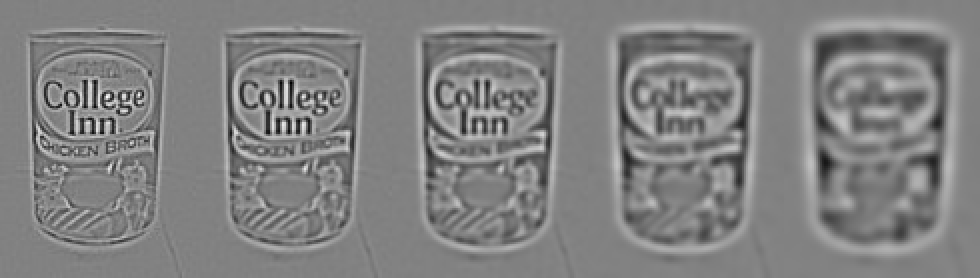
\includegraphics[width=.8\linewidth]{../results/q1_2.png}
    \caption{The DoG Pyramid of \code{model\_chickenbroth.jpg}}
    \label{fig:q1.2}
\end{figure}

\newpage

\subsection*{Q1.5}

Please see Figure.~\ref{fig:q1.5} for the detected keypoints of \code{model\_chickenbroth.jpg}.

\begin{figure}[h!]
    \centering
    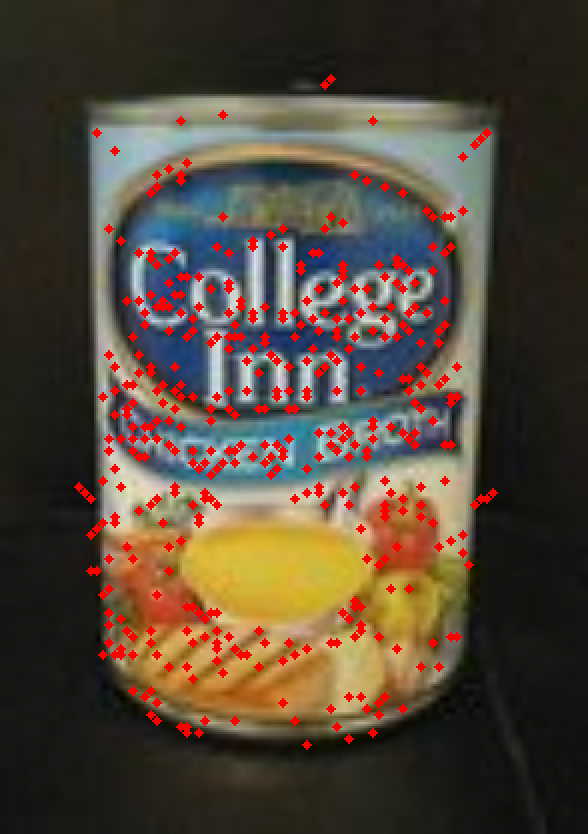
\includegraphics[width=.4\linewidth]{../results/q1_5.png}
    \caption{The detected keypoints on image \code{model\_chickenbroth.jpg}}
    \label{fig:q1.5}
\end{figure}

\newpage


\end{document}
